\documentclass[11pt]{sdm}
\usepackage{xcolor}
\usepackage{hyperref}
\definecolor{default-linkcolor}{HTML}{A50000}
\definecolor{default-filecolor}{HTML}{A50000}
\definecolor{default-citecolor}{HTML}{A50000}
\definecolor{default-urlcolor}{HTML}{A50000}
\hypersetup{
    colorlinks=true,
    linkcolor=default-linkcolor,
    filecolor=default-filecolor,
    citecolor=default-citecolor,
    urlcolor=default-urlcolor,
    breaklinks=true,
    pdftitle={Function placement for FaaS applications in the fog},
    pdfauthor={Volodia PAROL-GUARINO},
    pdflang={en},
    }

\usepackage{amsmath,amssymb,amsfonts}
\usepackage{algorithmic}
\usepackage{graphicx}
\usepackage{textcomp}
\usepackage{xstring}
\usepackage[inline, shortlabels]{enumitem}
\usepackage[acronym]{glossaries}
\usepackage[backend=bibtex,style=ieee,natbib=true]{biblatex}
\usepackage{utf8}
\usepackage{lscape} 

\usepackage{diagbox} %table split headers
%\usepackage{longtable}
\usepackage{array}
%\usepackage{rotating}
\usepackage{eqparbox}
\usepackage{makecell, caption, booktabs}
\usepackage{booktabs}
\usepackage{pifont}

\usepackage{cleveref}
\crefname{section}{sec.}{secs.}
\Crefname{section}{Section}{Sections}
\Crefname{table}{Table}{Tables}
\crefname{table}{tab.}{tabs.}
%\newcommand{\crefrangeconjunction}{--}
% \newcommand{\creflastconjunction}{, and } % optional, for "Oxford comma"
% \crefrangelabelformat{enumi}{#3#1#4--#5\crefstripprefix{#1}{#2}#6}
% {enumi}{first}{second}{middle}{last}
% \crefmultiformat{enumi}%
% {(items~(#2#1#3)}{ and~#2#1#3}{, #2#1#3}{ and~#2#1#3)}

% \crefrangemultiformat{enumi}%
% {(items~#3#1#4--#5#2#6}{ and~#3#1#4--#5#2#6)}{, #3#1#4--#5#2#6}{ and~#3#1#4--#5#2#6)}


\DeclareNameFormat{labelname:poss}{% Based on labelname from biblatex.def
  \nameparts{#1}% Not needed if using Biblatex 3.4
  \ifcase\value{uniquename}%
    \usebibmacro{name:family}{\namepartfamily}{\namepartgiven}{\namepartprefix}{\namepartsuffix}%
  \or
    \ifuseprefix
      {\usebibmacro{name:first-last}{\namepartfamily}{\namepartgiveni}{\namepartprefix}{\namepartsuffixi}}
      {\usebibmacro{name:first-last}{\namepartfamily}{\namepartgiveni}{\namepartprefixi}{\namepartsuffixi}}%
  \or
    \usebibmacro{name:first-last}{\namepartfamily}{\namepartgiven}{\namepartprefix}{\namepartsuffix}%
  \fi
  \usebibmacro{name:andothers}%
  \ifnumequal{\value{listcount}}{\value{liststop}}{'s}{}}
\DeclareFieldFormat{shorthand:poss}{%
  \ifnameundef{labelname}{#1's}{#1}}
\DeclareFieldFormat{citetitle:poss}{\mkbibemph{#1}'s}
\DeclareFieldFormat{label:poss}{#1's}
\newrobustcmd*{\citepossalias}{%
  \AtNextCite{%
    \DeclareNameAlias{labelname}{labelname:poss}%
    \DeclareFieldAlias{shorthand}{shorthand:poss}%
    \DeclareFieldAlias{citetitle}{citetitle:poss}%
    \DeclareFieldAlias{label}{label:poss}}}
\newrobustcmd*{\citeposs}{%
  \citepossalias%
  \textcite}
\newrobustcmd*{\Citeposs}{\bibsentence\citeposs}
\newrobustcmd*{\citeposss}{%
  \citepossalias%
  \textcites}

\addbibresource{biblio.bib} %added
\def\BibTeX{{\rm B\kern-.05em{\sc i\kern-.025em b}\kern-.08em
    T\kern-.1667em\lower.7ex\hbox{E}\kern-.125emX}}


\renewcommand{\arraystretch}{1.7}


%numeroter les pages
\pagestyle{plain}

\title{Function placement for FaaS applications in the fog}
\author{Volodia \textsc{Parol-Guarino}}
\supervisorOne{Nikolaos \textsc{Parlavantzas}}
\supervisorTwo{First\_Name \textsc{Name} of your second supervisor}
\team{MYRIADS}
%One of:
% ens-Rennes  esir    insa-rennes   rennes1  
% enssat    logoUbs   tsupelec
%here rennes1 for example
\school{insa-rennes}


% the domain should be one or two of:
% Technology for Human Learning 
% Artificial Intelligence 
% Computer Arithmetic
% Hardware Architecture
% Automatic Control Engineering
% Bioinformatics 
% Biotechnology
% Computational Complexity 
% Computational Engineering, Finance, and Science
% Computational Geometry 
% Computation and Language 
% Cryptography and Security 
% Computer Vision and Pattern Recognition
% Computers and Society 
% Databases 
% Distributed, Parallel, and Cluster Computing 
% Digital Libraries
% Discrete Mathematics 
% Data Structures and Algorithms 
% Embedded Systems 
% Emerging Technologies 
% Formal Languages and Automata Theory 
% General Literature 
% Graphics 
% Computer Science and Game Theory 
% Human-Computer Interaction 
% Computer Aided Engineering 
% Medical Imaging 
% Information Retrieval 
% Information Theory 
% Ubiquitous Computing 
% Machine Learning
% Logic in Computer Science 
% Multiagent Systems 
% Mobile Computing
% Multimedia
% Modeling and Simulation 
% Mathematical Software 
% Numerical Analysis 
% Neural and Evolutionary Computing 
% Networking and Internet Architecture 
% Operating Systems 
% Performance 
% Programming Languages 
% Robotics 
% Operations Research
% Symbolic Computation 
% Sound
% Software Engineering 
% Social and Information Networks 
% Systems and Control 
% Image Processing 
% Signal and Image Processing 
% Document and Text Processing
% Web
\domain{Domain:  Distributed, Parallel, and Cluster Computing -- Fog: Cloud after the edge}

%write your abstract here
\abstract{write your abstract here}


% \makeglossaries   
\newacronym{FaaS}{FaaS}{Function-as-a-Service}
\newacronym{PaaS}{PaaS}{Platform-as-a-Service}
\newacronym{SaaS}{SaaS}{Software-as-a-Service}
\newacronym{IaaS}{IaaS}{Infrastructure-as-a-Service}
\newacronym{OSS}{OSS}{Open-Source Software}
\newacronym{AI}{AI}{Artificial Intelligence}
\newacronym{SLA}{SLA}{Service Level Agreement}
\newacronym{SLO}{SLO}{Service Level Objectives}
\newacronym{VM}{VM}{Virtual Machine}
\newacronym{PAPS}{PAPS}{Partitioning, Allocation, Placement, and Scaling}
\newacronym{IoT}{IoT}{Internet of Things}
\newacronym{SEP}{SEP}{Serverless Edge Platform}
\newacronym{IoV}{IoV}{Internet of Vehicules}
\newacronym{RSU}{RSU}{Road-Side Unit}
\newacronym{VCG}{VCG}{Vickrey-Clarke-Groves}
\newacronym{SDN}{SDN}{Software-Defined Networking}
\newacronym{LI}{LI}{Least-Impedance}
\newacronym{RP}{RP}{Random-Proportional}
\newacronym{RR}{RR}{Round-Robin}
\newacronym{LaSS}{LaSS}{LAtency Sensitive Serverless}
\newacronym{LLA}{LLA}{Low Latency Application}
\newacronym{QoS}{Qos}{Quality-of-Service}    
\newacronym{MEC}{MEC}{Multi-access Edge Computing}
\newacronym{ACO}{ACO}{Ant Colony Optimization}
\newacronym{ETSI}{ETSI}{European Telecommunications Standards Institute}
\newacronym{NFV}{NFV}{Network Function Virtualization}
\newacronym{GPU}{GPU}{Graphical Processing Unit}
\newacronym{QoE}{QoE}{Quality of Experience}
\newacronym{SoC}{SoC}{System-on-a-Chip}
\newacronym{ISP}{ISP}{Internet Service Provider}

\begin{document}
\maketitle

%*****************************************************************%

\section{Introduction}
%\begin{itemize}
% \item Introduce \gls{FaaS} paradigm (as an extension of serverless?)
% \item Serverless is still improving, especially on the biggest problems (eg. coldstart) where even the base technologies are starting to be questioned and concurrenced by faster and more precise technologies \citet{hykes_solomon_2019}
% \item Introduce Fog, along with a word about \gls{MEC} and cloudlets
% \item indicated sections where to find more details
% \item {List of open questions from \citet{kjorveziroski_iot_2021}
%       \begin{enumerate}
% 	      \item Scheduling
% 	      \item deployement
% 	      \item performance
% 	      \item cold start
% 	      \item vendor lock-in
% 	      \item security \& isolation
% 	      \item improvement to function chaining / combination (preferrably even)
% 	      \item support for hardware acceleration (GPU, AI)
%       \end{enumerate}
% \item { Another approach is contributed by \citet{xie_when_2021}. They explore the challenges from the perspective of networking, as this is the main layer that enables the Fog to exist in the first place. It is relevant because of \gls{NFV} and \gls{SDN} and the relative closeness of \gls{MEC}
%       \begin{enumerate}
% 	      \item service deployement
% 	      \item resource awareness and service discovery
% 	      \item service scheduling
% 	      \item incentive mechanism
% 	      \item exceptions and failure recovery
%       \end{enumerate}
%       }
% \item Usually papers about IoT because these kind of devices are expected to take over
% \item Research on the metrics to optimize as well as the way to optimize them
% \item This issue is a problem because strategies needs to precisely account for this such as \citeposs{kaffes_centralized_2019} work that emphasizes about predictabability of performances. To do so they defend a centralized approaches instead of decentralization. Main causes: burstiness of the load + cold start that need to be managed and orchestrated at a higher level
% \item cold-start also a problem, especially in a constrained Fog node.
% \item Need to introduce to the ``big question''. Where to place \gls{FaaS} in the Fog, in a place that spans from the emitter to the cloud itself, while traveling a number of heterogeneous nodes.
% \item Explain in what it is difficult to solve (heterogeneity, dynamism, ownership, geographical distributions, etc.)
%       }

%Fog answers to a number of challenges posed by the Cloud and current models \cite{chiang_fog_2016}: 
%\begin{enumerate*}[(a)]
%	\item \emph{low / deterministic latency requirements} for real-time applications ;
%	\item \emph{network bandwidth constraints} that cannot be relieved ;
%	\item \emph{resource-constrained} producers not able to process locally ;
%	\item \emph{uninterrupted service} accidental or not ;
%	\item \emph{security}, switch away from limited perimeter-based approaches to protect many devices, constrained, trusted or not, all without disruptions.
%\end{enumerate*}

% \end{itemize}

Exploitation of computing power at the Edge of networks is a step towards real-time applications \cite{rausch_towards_2021,lin_cloudfog_2017}, \gls{IoT}, data and energy efficiency \cite{ieee_standards_association_smart_2018}, data-exploitation through analysis \cite{openfog_consortium_real-time_2018} or caching \cite{ma_understanding_2017}.

Such an evolution is currently undergoing thanks to the emergence of models such as the \gls{ETSI} specified \gls{MEC} and advances like \gls{NFV} and \gls{SDN}. However, \gls{MEC} strictly stops at just the edge of teclo's networks. Fog redefines the frontier. First of all, the concept utilizes all resources along the things-to-Cloud continuum: each an every computing enable node between the data producer (\gls{IoT} devices, smartphones, etc.) and the Cloud will be exploited. Even the Cloud is part of the model, because of its power and central nature.

Fog will require a computing model to execute tasks. Such models are in the likes of microservices, stream-processing or serverless. The latter is the explored one here. Especially one of its subsets: \gls{FaaS}. This model divides an application in small-scale ``function'' slices. It is easy to understand a function as to be a stateless unit of processing. As such, it requires to be downloaded, executed and fed data. An analysis is conducted in order to identify current challenges, and possible working directions.

Existing platforms usually focus on latency and resource management to apply their scheduling strategies. However, less work has been produced about the transit of data -- input, output, and the function themselves. Another void is the lack of contracts that would enable a developer to have guarantees, eg. in the case of latency-sensitive heart-attacks detection applications provisioned in the Cloud because another function processing \gls{IoT} filtering was executed instead.
For this reason, particular attention has been paid to auctions. Such mechanisms enable the expression of value contained in the function execution, data, localization, etc. One ambition would be to represent a developer's function value as truthfully as possible for decentralized scheduling to take place and make globally the best decisions.

Other identified challenges -- or opportunities -- reside in \gls{FaaS} limitations. The worst known being the ``cold-start'' problem, ie. a delay caused by the instantiation of the runtime of the business code's environment. However, check-pointing methods could be employed to mitigate this problem, as well as good caching strategies to avoid useless multiplication of that delay.

The report is then divided as follows. \Cref{sec:background} further differentiates Fog and \gls{MEC}, discuss \gls{FaaS} and provides applications examples. \Cref{sec:platforms} present \gls{FaaS} platforms. Then \cref{sec:placement} discuss litterature on function placement in the Fog. Finally, \cref{sec:curated} approaches a curated list of identified challenges from the previously examined literature.


\section{Background}
\label{sec:background}

\subsection{Fog and related concepts}

Four concepts currently coexists. One defines Fog. They all share a same basis of both benefits and challenges of developing and utilizing the Edge -- and beyond \cite{george_nanolambda_2020}.

\begin{description}
	\item[Edge Computing] defines \emph{exclusively} the utilization of computing resources located at the edge of networks. The user (event producer) is geographically far from the core/Cloud in the Cloud-centered model. Having access to closer resources could alleviate latencies as much as it can improve \gls{QoS} and \gls{QoE} of applications.

	\item[Cloudlets] first appeared in \cite{satyanarayanan_case_2009} issued in \citedate{satyanarayanan_case_2009}. The metaphor is to move part of the Cloud as close to the user as possible, eg. service it in the wireless LAN he is connected to. In this architecture, the mobile user exploits a \gls{VM} quickly instantiated on demand. It allows him to utilize a trusted, resource-rich computer -- or cluster. This computer -- a mobility enhanced, small-scale, cloud data-center located at the edge -- is required to be ``well-connected'' to the Internet and available for use by nearby mobile devices. As cloudlets are distributed geographically, one great preoccupation has been how to deal with the \gls{VM} instances as the mobile user changes location.

	\item[\acrfull{MEC}] was first introduced under the name \emph{Mobile} Edge Computing. It is an \gls{ETSI} standard backed by Huawei, IBM, Intel, Nokia Networks, NTT DoCoMo, Vodafone, and other companies. The name changed to emphasize on the relevance of this technology for all networks -- and not only the radio-based ones such as 5G networks. The standard is a way to unite both the telco an IT-Cloud worlds \cite{dahmen-lhuissier_etsi_nodate-1} as it was first though to implement Cloud at 5G base stations. It enables applications to be hosted in a multi-vendor, multi-access, edge-only computing environment -- ``on-top'' of mobile network elements. This is enabled by other emerging technologies such as \gls{NFV} \footnote{\acrfull{NFV} is the ability for networking equipment to rely on software functions rather than hardware ones \cite{redhat_what_2019}. It leverages virtualization as a way towards agility. Use cases include DHCP, firewall, and general execution of routing components, all virtualized.} and \gls{SDN} \footnote{\acrfull{SDN} dynamically routes requests in a centralized fashion. It separates the control plane from the data plane, thus sailing away from classical routing where all nodes participate in both decision-making and data handling \cite{redhat_what_2019}. Centralization helps to achieve optimal routing, especially at the scale of a network operator.}. \gls{MEC} is proposed as a trusted vertical solution for \gls{IoT} and mission critical solutions. \gls{MEC} applications make use of virtualization to be purely software byproducts. The virtual infrastructure also includes a data plane for routing among all the connected networks (applications, internal and external). A gateway decides whether a request is granted or not. The accepted request is then forwarded to the orchestrator for further processing. \gls{MEC} works in a centralized way arranged around that orchestrator. It knows the topology, available resources and \gls{MEC} services provided.

	\item[Fog computing] is a horizontally distributed architecture aiming to bring both the data plane and the control plane closer to the end-user -- the event producer -- by exploiting all the computing-enabled places along the cloud-to-things continuum. In other words, Fog creates an immersive distribution of computing, where task execution occurs geographically near the producer, while keeping centralized-dependent heavy processes treated in the Cloud, where it is best handled. Fog is different from the previous two other edge-only approaches as it provides tools for distributing, orchestrating, managing and securing both resources and services across networks and devices living in the continuum, while also thriving there.

		A Fog node has multiple functions, including but not limited to: networking, computing, accelerating (using \gls{GPU}, etc.), storing and control. It can be worked as a mesh.
		%	 Fog nodes are not conceived to be present at the teclo's operator Edge in the first place, in contradiction to the \gls{MEC} model.

		\begin{figure}[t]
			\centering
			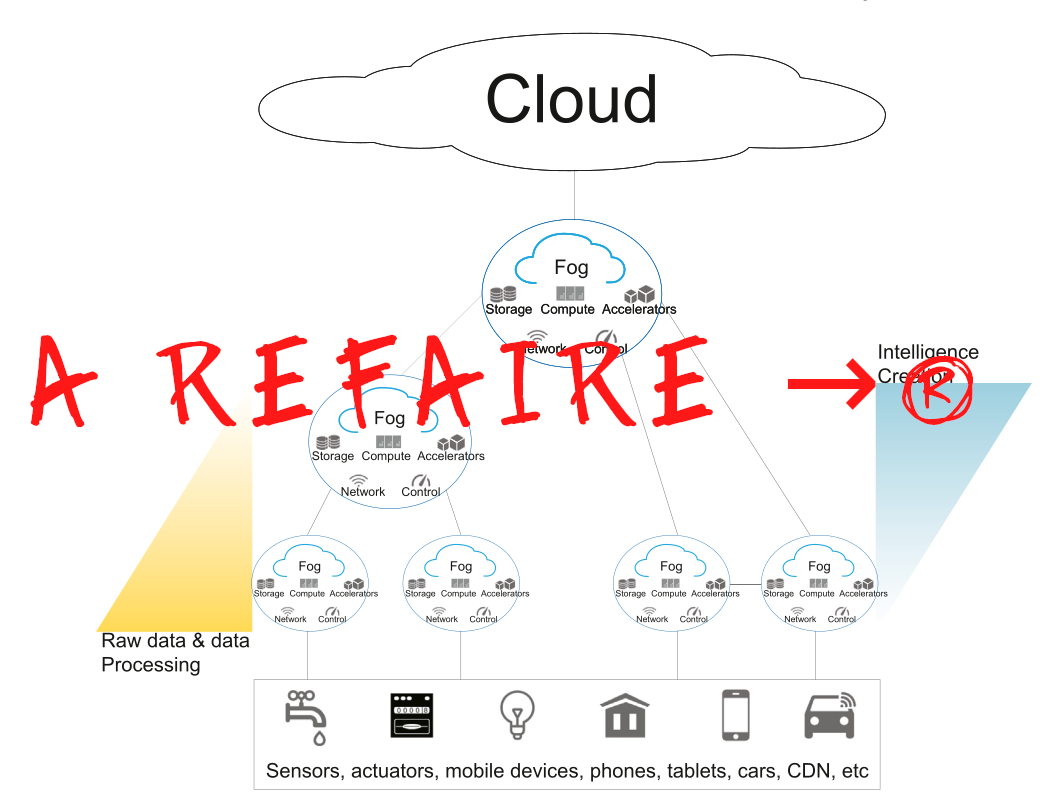
\includegraphics[width=0.75\textwidth]{./assets/FogArchi.png}
			\caption{A typical intelligence creation, hierarchical, architecture based on Fog computing}
			\label{fig:fog_archi}
		\end{figure}

		Fog presents a natural hierarchical organization. Fog nodes at the very edge are usually lighter on processing capabilities and may be reserved to tasks such as filtering or simple transformations. Getting closer to the Cloud, the value of the processing of each node will increase, as much as the intelligence creation will, cf. \cref{fig:fog_archi}.

		%	Fog answers to a number of challenges posed by the Cloud and current models \cite{chiang_fog_2016}: 
		%	\begin{enumerate*}[(a)]
		%		\item \emph{low / deterministic latency requirements} for real-time applications ;
		%		\item \emph{network bandwidth constraints} that cannot be relieved ;
		%		\item \emph{resource-constrained} producers not able to process locally ;
		%		\item \emph{uninterrupted service} accidental or not ;
		%		\item \emph{security}, switch away from limited perimeter-based approaches to protect many devices, constrained, trusted or not, all without disruptions.
		%	\end{enumerate*}

		Back in \citedate{bonomi_fog_2012}, Cisco introduces the key characteristics of Fog thanks to \citeposs{bonomi_fog_2012} paper:
		\begin{enumerate*}[(i)]
			\item low-latency and location awareness ;
			\item wide-spread geographical distribution ;
			\item mobility ;
			\item very large number of nodes ;
			\item dominance of Wireless access ;
			\item Real-time and streaming applications as first citizens ;
			\item heterogeneity.
		\end{enumerate*}
		The Fog initiative is now backed by the OpenFog Consortium \cite{ieee_standards_association_ieee_2018} constituted of ARM, Cisco, Dell, Intel, Microsoft and Princeton University \cite{chiang_fog_2016}.
\end{description}

The benefits are similar for all the paradigms \cite{ahmed_fog_2019, ai_edge_2018}:
\begin{enumerate*}[(1)]
	\item latency reduction ;
	\item bandwidth optimizations ;
	\item computational offloading ;
	\item privacy and security through on-premise exploitation ;
	\item service management as a middleware ;
	\item edge-device monitoring ;
	\item energy efficiency-enabling vector ;
	\item cost savings through platform acquisition ;
	\item content caching.
\end{enumerate*}

%\begin{figure}[t]
%	\centering
%	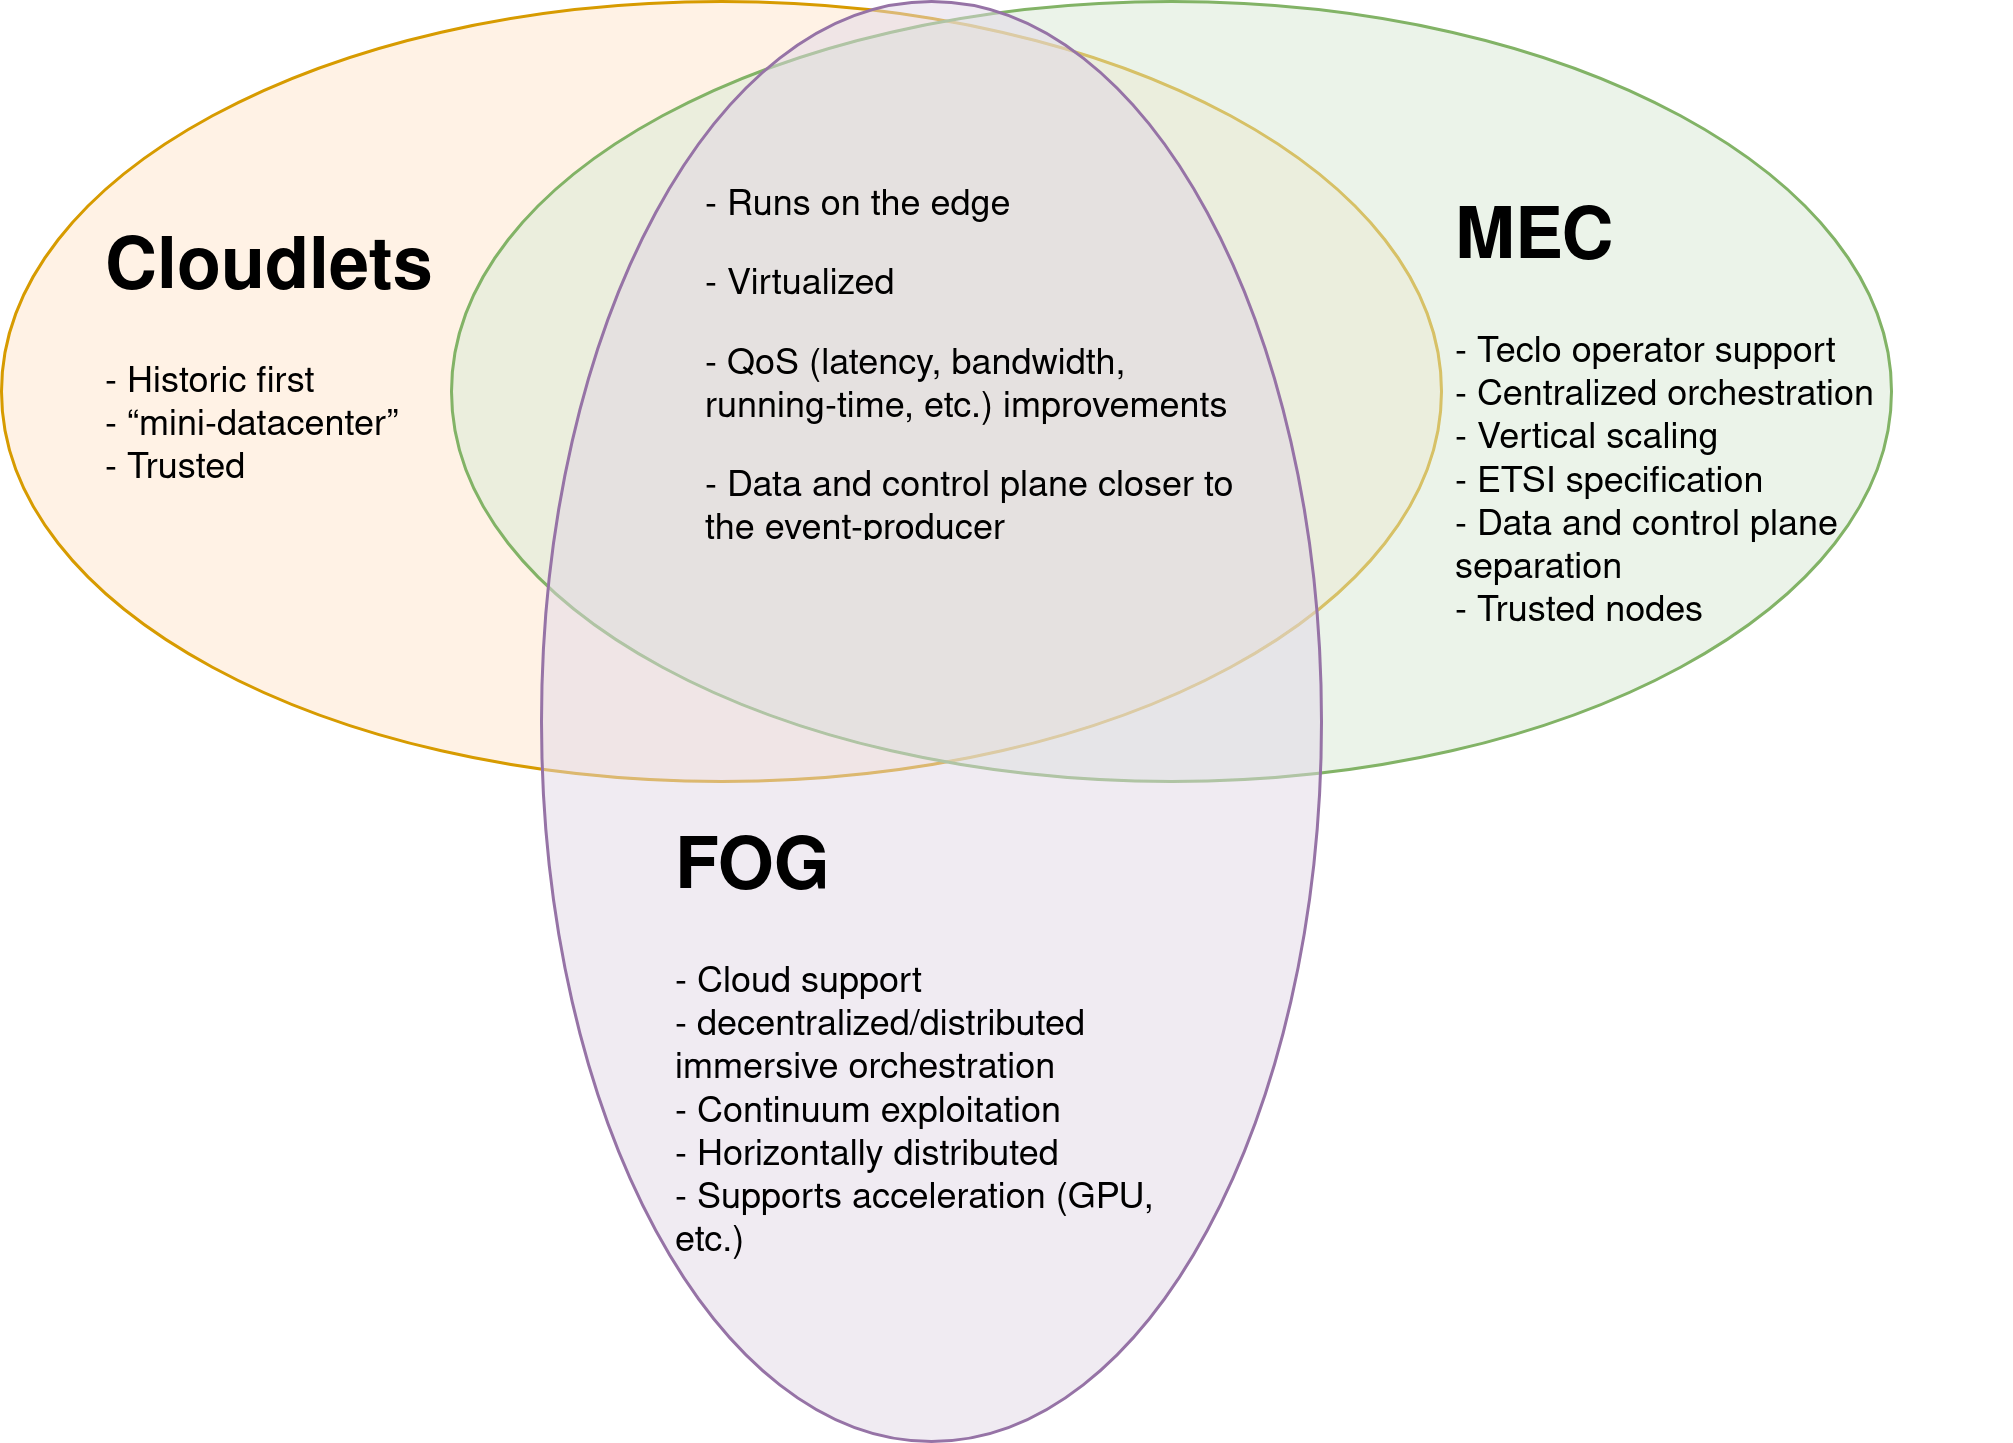
\includegraphics[width=0.75\textwidth]{./assets/CloudLetsVMECvFog.drawio.png}
%	\caption{Key differences between all the edge -- and beyond -- paradigms}
%	\label{fig:fogVall}
%\end{figure}

While all these concepts focus on exploiting the edge of the networks to achieve similar goals constrained by similar challenges, only Fog exploits all the continuum and considers Cloud as much as the edge -- and further than it. However, only \gls{MEC} posses a specification as of 2022. The Fog Consortium acknowledges it and recommends the Fog initiative contributors to avoid duplication of efforts and focus on aspects not optimized by other approaches.

Another point of relevance for \gls{MEC} are propositions like \citeposs{chaudhry_improved_2020}. Merging \gls{MEC} and \gls{NFV} together towards a single mighty serverless model in order to improve both paradigms.

In the long term, the consortium hopes liaisons will form to bring the industry to a common ground \cite{ieee_standards_association_ieee_2018}.
%The key differences of those different paradigms are highlighted in figure\ref{fig:fogVall}.

\hypersetup{linkcolor=}
\subsection{Serverless and \acrfull{FaaS}}

Relative to the novelty of the Fog concept, the computing paradigm such a technology would follow is not yet decided. \gls{FaaS} is a Cloud-native technology ; would its potential hold in the case of Fog? \ref{sec:literature_review} is full of examples going that way.

\gls{FaaS} is a concept that allows the developer to only focus on the business logic and not the provisioning of the resources \cite{redhat_what_2020}. As its name suggest, the base unit is a function -- like the one we use everywhere in computing. This is where its resemblance with micro-services shines the most, because the application is cut in those base units, usually stateless. This is where similarity stops because provisioning, scaling, capacity management is not the developer's burden anymore, and the Cloud provider is happy to inherit it. It allows him to then optimize its architecture, costs, configuration and enable a global management much more fine-grained than with \gls{PaaS} or \gls{IaaS}.

It should not be confounded with \emph{serverless} which is its parent concept. \gls{FaaS} concentrates on an event-driven computing focused aspect. Once an event triggers the platform, the function is started. This is where serverless is much more general, because it comprises compute, storage, database, messaging, api gateways, etc. in its scope. The rest is still the same: configuration, management and billing are invisible for the user \cite{ibm_faas_2019}.

In the case of Fog, serverless and \gls{FaaS} means resource-constrained environments decide how to manage their resources and only handle small slices of one's application because of the division in functions \cite{bermbach_auctionwhisk_2021}.

The introduction of serverless and \gls{FaaS} contribute to new challenges, especially mixed with Fog. To name the most meaningful \cite{kjorveziroski_iot_2021}:
\begin{enumerate*}
	\item \emph{cold starts}, the time spent preparing the runtime before executing the function in it ;
	\item \emph{Scheduling} and handling different frequencies of execution, provisioning and halting ;
	\item \emph{deployement}, where to store the functions, their data, their states, etc. ;
	\item \emph{performance} and the technical underlying difficulties caused by languages, virtualization techniques (\gls{VM}, containers, WASM) ;
	\item \emph{vendor lock-in} and dependency on only one provider ;
	\item \emph{security \& isolation} that is especially true under resource constraints \cite{maurice_hello_2017} ;
	\item \emph{improvement to function chaining / combination} with non-trivial ways to manage performance (latency, etc.) and costs \cite{elgamal_costless_2018} ;
	\item \emph{support for hardware acceleration (GPU, AI)}.
\end{enumerate*}

%takes the benefits of that originates from limitations of trends like \gls{SaaS}, \gls{PaaS}, etc. and micro-services.
%
%Serverless is a Cloud-originated paradigm. It is another *-as-a-Service that originates from limitations of trends like \gls{SaaS}, \gls{PaaS}, etc. and micro-services that are well recognized among the industrial community. It can be viewed as an evolution while it actually restrict the control of the developer. The base unit is the \emph{function}, as in plain-old regular function of most of the languages. Here, this code is the sole responsibility of the developer, he needn't to worry about the underlying provisioning or infrastructure. This is an evolution because making those responsibilities the provider's mean he will be able to scale, optimize and provision resources without restrictions. Effectively this means a simpler approach to the Cloud with less no worries outside the developer's core job, which is not to know how to provision his application in a datacenter.

%\subsection {Context}
%\begin{itemize}
%	\item introduce serverless in more depth
%	\item Introduce \gls{FaaS}
%	\item About serverless, \citeposs{elgamal_costless_2018} work about AWS Greengrass shed the light on the ability to maintain serverless applications under a certain latency threshold by utilizing a fusion-placement algorithm that finds non-trivial memory and placement configurations.
%\end{itemize}

\subsection {Applications}

\begin{table}[t]
	\fontsize{10}{8}\selectfont
	\begin{tabular}{@{} p{3cm}|p{12cm} @{}}
		Economic sector & Description
		\\[2ex]
		\cmidrule[1pt]{1-2}
		%		Transportation 
		%		& LiveMap provides fine-grained details about road conditions thanks to vehicular updates \cite{hu_live_2017}.
		%		\\
		%		Health 
		%		& Stroke detection thanks to Fog-distributed fall-detection algorithms, stroke mitigation and splits task detection between smartphones and Cloud servers \cite{hu_survey_2017}.
		%		\\
		Caching
		                & Video streaming file caching in edge networks \cite{ma_understanding_2017}.
		\\
		Augmented Reality
		                & Track and display the position of physical objects not in the physical field of view of a user in the context of smart cities. The object are displayed on smart glasses. Real-time processing is possible thanks to edge nodes processing neighboring camera feeds \cite{rausch_towards_2021, rausch_cognitivexr_2020}.
		\\
		Entertainment
		                & Avoid the requirements of installing games on the computers and utilize Fog nodes with hardware acceleration to render game videos \cite{lin_cloudfog_2017}.
		\\
		Smart cities
		                & Integration of Fog nodes in smart buildings would provide the architecture for new use cases towards better energy efficiency, lower operational costs, etc. thanks to the exploitation of existing sensors in buildings \cite{ieee_standards_association_smart_2018}.
		\\
		%		Supply chains 
		%		& Create the ability for delivery drones to collaborate and make operational changes and adjustments in response to anomalies \cite{openfog_consortium_out_2018}.
		%		\\
		%		Smart factories 
		%		& Make smarter brewing thanks to intelligent nodes able to scale and replicate key functions to a production process with large fluctuations in demand periods \cite{openfog_consortium_process_2018}.
		%		\\
		Energy, civil, environment industries
		                & Enable real-time subsurface monitoring to better understand subterranean dynamics that would pose threat or make opportunities for oil, gas and geothermal exploitation and exploration \cite{openfog_consortium_real-time_2018}.
		\\
		%		Smart grid 
		%		& Allow the processing of home-based \gls{IoT} closer to the home in question rather than processing the data in another country's Cloud datacenter \cite{chen_design_2018}.
		%		\\
		%		Agriculture 
		%		& Enable a high-precision smart irrigation system for agriculture thanks to optimizations of the irrigation system computed all along the Edge-to-Cloud continuum \cite{noauthor_swamp_nodate}.
		%		\\
		%		Security (IT, physical) 
		%		& Enable a hardware accelerated antivirus to be executed remotely on a close Fog node rather than on the constrained smartphone where it would normally not be able to \cite{deyannis_enabling_2018}.
		%		\\
		\cmidrule[1pt]{1-2}
	\end{tabular}
	\caption{\label{tab:applications}Insight about Fog applications \cite{ahmed_fog_2019}}
\end{table}

Fog is envisioned as a way to avoid sending massive amounts data far away and is predicted to be efficient into bringing low-latency and even real-time applications to life \cite{ahmed_fog_2019}. However, no general Fog platform is yet publicly known. \citet{ahmed_fog_2019} have presented an in-depth review of applications, some of their examples are described in \ref{tab:applications}.

\citet{ahmed_fog_2019} also identifies Fog deployment models, similar to the Cloud landscape. Fog can be declined into
\begin{enumerate*}[(a)]
	\item \emph{private Fog} with execution exclusivity for one user, as well as the hardware's responsibility;
	\item \emph{public Fog}, the opposite, usable by the grand public ;
	\item \emph{community Fog}, exclusive to the member of a community ;
	\item \emph{hybrid Fog}, which is a mix of all the previous and usually serves scaling purposes.
\end{enumerate*}
This variety of models caused by accessibility-related constraints on physical Fog nodes indicate a need for cooperation of the nodes, ie. bring the ability of connecting private nodes with public/community ones using a standard set of protocols and market methods to trade computing powers and resources in real-time. Some propositions even consider the creation of an edge network not relying on \glspl{ISP} \cite{bermbach_towards_2021}.

\section{Platforms}
\label{sec:platforms}

A variety of platforms exist to accommodate Fog with the current state of industrial applications. Most of them are focused on a private usage. The node is owned by only one user that exploit a small park of nodes for his only benefit. However, many options -- especially the \gls{OSS} ones -- offer the feature of modification and extension needed to bring the Fog paradigm to the next step in an open/reproducible research manner. For now, most of these platforms are derivative of successful Cloud-based ones, this state-of-the-art leads to technical challenges of running this kind of platform in a resource-constrained fog node.

%During this internship, the light will be shed on \gls{OSS} platforms, as they are easier to use, have a public community and documentation linked to the underlying code, and are the only option compatible with open/reproducible research \cite{kjorveziroski_iot_2021}.

%\begin{itemize}
%    \item Several choices
%    \item Main question is to either use already developed code to adapt to the Fog, or to create a new interoperable platform
%    \item The focus is on adaptability, as Fog encompass and extends Cloud
%    \item The technical problem is then to adapt the technology for a new, more demanding platform.
%    \item a distinction can be made between commercial extension and \gls{OSS} extension. The later one can mitigate the vendor lock-in problem described by \citet{kjorveziroski_iot_2021}, and if not, is the only category compatible with open/reproducible research.
%\end{itemize}

\subsection{Commercial focus}

These proprietary platforms are published by cloud giants. The list include, but is not limited to: Amazon AWS Greengrass \cite{noauthor_aws_nodate}, Microsoft Azure IoT edge \cite{noauthor_iot_nodate} and Google Iot core \cite{noauthor_cloud_nodate}. Usually these platforms connect to their editor's cloud as another premium service offered from their panel. The use is then exclusive to the developer connecting them. The functionalities offered can be close to \gls{FaaS}, but triggered and processed closer to the data source \cite{elgamal_costless_2018}.

%\begin{itemize}
%    \item Existing offers from cloud giants, such as  \citeposs{elgamal_costless_2018} work emphasize on cost optimization of serverless computations spanning from the cloud to the very edge where Greengrass can be executed on a node by a user. Though the authors use what they called an edge node, it actually corresponds to the characteritics of a fog node placed at the edge of their network.
%    
%    %Durable functions = Greengrass for microsoft, Azure IoT edge ?
%\end{itemize}

\hypersetup{linkcolor=}
\subsection{\acrfull{OSS}}
\gls{OSS} projects offer more transparent platforms. This is the case of Apache OpenWhisk \cite{noauthor_apache_nodate}. It has been started by IBM and then made publicly available through an Apache 2.0 licence. This kind of platform is preferred in the era of open-research for obvious reasons as well as limiting an existing Cloud problem: vendor lock-in \cite{kjorveziroski_iot_2021}. Adaptations have been made to retain the benefit of the source code while running on the more resource-constrained Fog nodes. The project is named Lean OpenWhisk \cite{breitgand_lean_2018}.

Another axis of development is focused on a variety of Kubernetes extensions \cite{bocci_secure_2021}, to name a few: Fission, Kubeless, Knative, OpenFaaS, Nuclio.

Other works have focused on the opposite problem. Instead of adapting the Cloud paradigm to the Edge, edge-native platforms have started to appear. \citet{pfandzelter_tinyfaas_2020}] shows better performances than Lean OpenWhisk. While the work is impressive, could it ever reach the industrial development level of platforms such as OpenWhisk or Kubernetes once their complete adaption will be achieved? \citeposs{george_nanolambda_2020}'s NanoLambda is another mighty small platform placed at the edge. Thought not compared, it would extend the reach of Fog to Clusters of IoT devices by making devices such as Espressif's ESP8266 \gls{SoC} \cite{noauthor_esp8266_nodate} able to run \gls{FaaS} platforms. Thus enabling a closer layer of processing right inside IoT networks.

\section{Placement}
\label{sec:placement}

\subsection{Literature review \label{sec:literature_review}}

As previously introduced, the novelty of Fog research makes it hard to compare the landscape. To fix such a problem, surveys are conduced, such as \citeposs{bocci_secure_2021}.

%They introduce \cite{cheng_fog_2019, baresi_paps_2019, baresi_towards_2019, cicconetti_decentralized_2021}\\ % mortzavi + perssons

\begin{description}
	\item[\citet{cheng_fog_2019}] defines \textit{Fog functions} as a new \gls{FaaS} platform. They note data locality is of ``paramount'' importance. Data are observed to be linked with variable
		\begin{enumerate*}[(i)]
			\item entity size ;
			\item entity refresh rate ;
			\item task complexity ;
			\item task running-time ;
			\item task priority ;
			\item task novelty.
		\end{enumerate*}
		The authors also identify what a data-intensive Fog framework should provide:
		\begin{enumerate*}[(a)]
			\item data discovery and routing fine-grained to the content of the data ;
			\item function triggering solely based on the availability of the input data ;
			\item dynamic placement of either data or code to the best processing place ;
			\item data dependency as function composition driver.
		\end{enumerate*}
		Nodes are edge-base or cloud-based. Discovery and orchestration is centralized onto a particular node. The orchestrator is aware of data flowing to its nodes. It then decides where to execute each function. Data is then routed to that node and processing takes place.

	\item[\citeposs{baresi_paps_2019}] \gls{FaaS} platform is focused on low-latency, data-intensive use cases. \cite{baresi_towards_2019} identify multiple challenges to the creation of a \gls{MEC} platform by the research community, it comprises
		\begin{enumerate*}[(i)]
			\item resource management ;
			\item placement \& migration of application components and services between platforms ;
			\item scheduling of computation and offloading from mobile and \gls{IoT} devices.
		\end{enumerate*}
		The paper defines a \gls{SEP} that answers a list of requirements:
		\begin{enumerate*}[(a)]
			\item low-latency computation offloading ;
			\item inter-platform collaboration to ensure \gls{SLA} deadlines ;
			\item latency optimization to enable real-time communications ;
			\item opportunistic data analysis for anticipation ;
			\item edge coordination to enforce location awareness ;
			\item Stateful partitions to extend \gls{FaaS} support.
		\end{enumerate*}
		The authors then proceed to create a prototype implementing each of those points. Their solution is deployed on OpenWhisk. They observe a need to reduce latency, especially in real-time scenarios.

		\citet{baresi_paps_2019, baresi_paps_2021} extend this work with the \gls{PAPS} platform while advocating for a decentralized approach to increase speed of control.
		The architecture is divided into three layers:
		\begin{enumerate*}[(1)]
			\item A supervisor node that knows the global topology. Its responsibility is to form communities of nodes ;
			\item A community is an aggregation of nodes having a latency under a defined threshold. It is in charge of making sure \glspl{SLO} are reached and \glspl{SLA} not violated. The functions processed by the community are allocated by a leader. This centralized approach avoids the need of a more complex protocol while using well known optimal centralized techniques ;
			\item Local nodes then receive the responsibility of their allocated resources back, along with the function execution and its \gls{SLO}. Its challenge is not to break it or other application's.
		\end{enumerate*} So each node actually micromanages its allocated functions and their fluctuations the best they can, while still respecting the leader's decision and global view.

		Following the theory, and after a promising simulation, \citet{baresi_paps_2021} implements \gls{PAPS} on top of Kubernetes and OpenFaaS. Their conclusion is their partitioning allows for guarantees that decentralized heuristics cannot provide, while still doable in practice, unlike a fully centralized architecture. They also point out they can handle highly fluctuating workloads while acknowledging reactivity of nodes is a challenge due to their use of containers.

		% TODO check if reference wiht function/FaaS, otherwise goodbye
		%	\item[\citet{lee_trustful_2020}] position themselves in the \gls{IoV} paradigm, where vehicles interact with \glspl{RSU} located alongside the roads. The authors note in this case the untrustworthy vehicles can be used as attack vectors to compromise both the stability and the data integrity of the service by attacking the trusted \glspl{RSU}. Their contribution is a platform based on allocations decided by a one-shot version of the \gls{VCG} auction scheme named ``the Hungarian method'' \footnote{The ``the Hungarian method'', while ensuring one-to-one assignment of computing resources, finds the lowest cost way to divide the said resources \cite{wikipedia_hungarian_2021}. In \cite{lee_trustful_2020}, minimizing the cost is equivalent to a minimization of utilities, meaning the resources are strictly utilized to the necessary.}. Vehicles are bidding on computing resources made available by the \glspl{RSU}, or their adjacent neighbors. It is optimal for vehicles to bid their true utilities. If they do so, the resource assignment is fair. Results and purchased service times of transactions are secured using a tweaked and distributed blockchain that saves on both energy and computing power. The auction is initiated by the auctioneer -- a \gls{RSU} node -- and is broadcasted back to vehicles by adjacent nodes. Simulation of the platform concludes latency is negligible, while proportional to the number of connected vehicles. The second conclusion is that this method is deemed realizable.

	\item[\citet{cicconetti_decentralized_2021}] propose a decentralized platform to minimize response times while respecting short- and long-term fairness in stateless task assignations. Their platform does not extend to the Cloud and integrates by the standards of the \gls{MEC} model. An edge device is connected to an edge router that submits the stateless task request to an edge computer. The router decides autonomously where to forward the task in his known pool of compute-enabled nodes. The router proceeds to
		\begin{enumerate*}[(a)]
			\item update path weights \label{cicconetti_weights} ;
			\item choose a destination \label{cicconetti_destination}.
		\end{enumerate*}
		\ref{cicconetti_weights} is achieved by measuring a rolling average of routed function response times submitted to computing nodes. A \gls{SDN} controller supervising the network is used to know and avoid congested paths. \ref{cicconetti_destination} has been tested on three different algorithms. Namely
		\begin{enumerate*}[(i)]
			\item \gls{LI} -- always select the minimum cost node \label{cicconetti_li} ;
			\item \gls{RP} -- selects a random node with a probability proportional to the weighted \cref{cicconetti_weights} path to that node \label{cicconetti_rp} ;
			\item \gls{RR} combines the proportional benefits of \cref{cicconetti_rp} with the greediness of \cref{cicconetti_li} \label{cicconetti_rr}.
		\end{enumerate*}
		\ref{cicconetti_rr} achieves both short- and long-term fairness, while \cref{cicconetti_rp} only the latter. \cref{cicconetti_li} is the worst performer.
		The authors conclude the \gls{SDN} plays a capital role in the system. Under load variations, performance is equally as good as in a regular distributed systems. Finally, exploration of hierarchical forwarding in a simulated test-bed with OpenWhisk offers interesting scalability perspectives.

		%	\item[\citeposs{wang_lass_2021}] \gls{LaSS} platform is based on queuing models to manage resources with an exclusive focus on latency sensitive computations in edge clusters. The platform aims at ensuring each function meet its \gls{SLO} deadlines. The platform differentiates two behaviors: the absence of resource pressure and its contrary, alongside overloads. 
		%	\textcolor{red}{Present what happens in pressure. Forgot to finish reading the article there...}
		%	Anyway, the platform will monitor its functions in order to balance provisioning between them, allocating reclaimed resources to under-provisioned functions. A prototype of the platform is implemented on top of OpenWhisk to conduct an experimental evaluation. It concludes .

	\item[\citeposs{tasiopoulos_fogspot_2019}] FogSpot allows the provisioning of heavily stateful \glspl{LLA} -- \glspl{VM} that can neither be migrated nor suspended -- on Fog nodes along the path of an Edge device's request to its default execution location: the Cloud. That way either the request is accepted and provisioned or, it is forwarded to another further node. If it only gets forwarded, it ends up executed in the Cloud.
		Each node hosts a trusted market. A \gls{LLA} request is also truthful bid that shows its willingness to pay per unit of time and is directly related to its \gls{QoS} gain that would be observed if the request was to be accepted and the application served on this particular node. Of course, the further the request is from the edge, the lower the bid and the utility gets, until it finally reaches 0 and the Cloud.
		Each node can either choose to maximize its revenue or its social welfare. Those strategies are reflected in the used Dutch auctions termination's conditions. Such auctions are employed to keep processing requests on the spot, without having to queue and to wait anywhere along the request's way. A depth analysis of executions is conducted by the authors and reveal the first strategy leads to more gain for the node's provider but with uncertainties on the prices when executed in a decentralized/uncoordinated way while the second one will try to fully exploit the capacity of the node and provide a stable solution in an uncoordinated space.

	\item[\citeposs{mutichiro_qos-based_2021}] contribution is STaSA, a scheduler developed for KubeEdge to be executed in a \gls{MEC} community of nodes: multiple nodes aggregated around a leader because of their proximity latency-wise, here thought to be in a server rack. The scheduler is introduced as a way to respect as much as possible applications' \gls{QoS} requirements. Other objectives are also considered: node utilization maximization, cost minimization (compared to standard Cloud) and service-time optimizations. This problem is NP-hard. STaSa is built upon the \gls{ACO} probabilistic model to place containers -- called functions throughout the article. The model has been tweaked, especially during the pheromone updates and calculations. In principle, ants are dispatched to the nodes to find the best suitable placement. On their way back they leave a pheromone trace. Its intensity/weight depends on a number of factors the ant found in the node (CPU/RAM utilization, latency, QoS, etc.). Termination is reached when either a threshold is reached or when the best placement is found: when the minimal cost is thought to have been found. Practical implementations showcase better results than baselines \gls{ACO} and First Come First served strategies.

	\item[\citet{palade_swarm-based_2020}] theorized the idea of using the \gls{ACO} meta-heuristic algorithm for function placement in \gls{MEC}. The content can be directly compared to \cite{mutichiro_qos-based_2021}. Noting that the first dates back to \citedate{mutichiro_qos-based_2021} whereas the latter is older by a year ( \citedate{palade_swarm-based_2020} ). However, \cite{palade_swarm-based_2020} concentrates explicitly on \gls{MEC}. They also succeed to show this approach leads to less overall latency. They argue this gain largely mitigates the failure to find an optimal load-balancing and a ``sub-second'' higher execution time.

	\item[\citet{rausch_optimized_2021}] introduce Skippy. This function scheduler is based on annotations present in the functions code, such as an indication of hardware specific dependencies. It assumes a lesser level of control about the cluster status and functions requirements as it is observed in practice in the industry. The author present their work as an improvement over the default greedy multi-criteria decision making Kubernetes online scheduler \footnote{An online scheduler has no knowledge of future arrivals.} algorithm. They add four new aspects -- functions:
		\begin{enumerate*}[(i)]
			\item \emph{LatencyAwareImageLocalityPriority} that favors nodes where access to the container registry is quick enough ;
			\item \emph{DataLocalityPriority} influence the location of the function based on the predicted data transfer ;
			\item \emph{CapabilityPriority} that is aware of hardware accelerations requirements for functions ;
			\item \emph{LocalityTypePriority} that favors Cloud or Edge placement if required by the user.
		\end{enumerate*}

		In a second part of their paper, the authors implement a simulator to optimize the weights of their scheduler at scale. Their implementation allow for a single code basis as the simulator calls the Skippy scheduler directly.

		Simulations are executed over different plausible scenarios generated by a topology synthesizer as no large-enough test-bed exists.

		Conclusion shows their work enables
		\begin{enumerate*}[(a)]
			\item locality-sensitive function placement resulting in a better utilization of the network bandwidth ;
			\item tradeoffs of execution cost with application latency have been observed ;
			\item improving placement quality is counterbalanced with scheduler performance loss.
		\end{enumerate*}

		%TODO maybe merge the two references, cf https://onlinelibrary.wiley.com/doi/full/10.1002/spe.3058 which is the newer version of the paper, so ...
	\item[\citet{bermbach_towards_2020}] are interested in the issue of function placement in multiple geo-distributed sites in Fog fashion. From their perspective, a serverless -- particularly a \gls{FaaS} approach -- is relevant because provisioning is done in small slices instead of full containers or \glspl{VM}. Additionally, moving functions back and forth between Cloud and the Edge is easier due to their stateless natures. Their framework will use an auction-based approach, as they argue this kind of approach showed success in the past.
		Bidding is done when developing the function. Two bids are attached
		\begin{enumerate*}[(a)]
			\item \emph{Data storage bid}, ie. the price the developer is willing to pay for a node to store his executable per unit of time ;
			\item \emph{Processing bid}, ie the price the developer is willing to pay per for a node to execute his function.
		\end{enumerate*}
		These bids would be dirigible towards a preference for Cloud, Edge or a preferred node. Accepted bids are then paid over a minimum price, as a surcharge. A second-price auction is deemed to be the better option here.

		The authors then proceed to prove this approach works by developing a simulator and conclude auction-based function assignation and storage are an efficient mechanism in Fog-enabled contexts where there is both a lack of processing and storage capacity.

		In an incremental journal, \citet{bermbach_auctionwhisk_2021} identify four constraints to implement this model:
		\begin{enumerate*}[(i)]
			\item auctions process in batches, there is a need of a window of time when the system estimates refusing functions is required ;
			\item storage space calculations do not depend on the number of functions but on their sizes, especially as their metadata is expected to grow after each execution ;
			\item estimating the number of supported concurrent function executions as some functions will be either under or over-provisioned ;
			\item a node is required to know its neighbors, especially the one leading the path towards the Cloud ; however, this needs to be achieved despite node failures and parameter changing over time.
		\end{enumerate*}

		Then the authors present a prototype named \emph{AuctionWhisk}, based on OpenWhisk (also supporting the \emph{Lean} flavor). They experiment on a limited setup consisting in an edge, an intermediary and a cloud node.

		%	\item[\citet{elgamal_droplet_2018}] propose a scalable, dynamic programming algorithm named DROPLET that partitions operations in \gls{IoT} applications across Edge and Cloud. The problem -- the application -- is modeled in a placement graph weighted according to the sum of the cost of
		%	\begin{enumerate*}[(i)]
		%		\item the queuing delay ;
		%		\item the execution time ;
		%		\item the transmision delay.
		%	\end{enumerate*}
		%	Simulation shows the scalability of the model in decent computational times.

\end{description}

Other methods also present active management of a node executing function, eg. reclaim resources or grant more, this is the case of \gls{LaSS} developed by \citet{wang_lass_2021}. More classical approaches are also taken, as \citeposs{elgamal_droplet_2018} DROPLET that uses an underlying graph optimization algorithm.

% Still need a platform able to bound latency = guarantees ? = like SLA of the Cloud ? -> reserve subset at a given price

% Depreciating licenses ? \cite{milgrom_redesigning_2017}

% only request to cloud ? what happens if latency constrained ? Does it have to pay more ? what if load?

% TODO explain \gls{VCG}
% TODO explain blockchain
% TODO explain KubeEdge
% Bulk Synchronous Parallel (BSP) as elaborated in [18] for Faas ?

% another problem : versionning of the nodes and their executed content
% another problem : do we take the user preference, in term of placement, energy (from Ayan Mondal, preprint emailed)

% Explain why Fog placement and FaaS placement cannot be separated from orchestration, because of the impact of each other

% cicconetti_decentralized_2021 has examples for applications + points out the need of a custom platform because of high overhead of K8S, etc.

% decentralized != distributed

% TODO check all the enumerated to add commas

\section{Curated list of unresolved problems}
\label{sec:curated}

%\newcommand{\tabred}{-4pt}
%\newcommand*\rot{\rotatebox[x=2cm]{90}}
\newcommand*\rot{\rotatebox{90}}
\newcommand*\OK{\ding{51}}
\begin{table}[t] \centering
	\fontsize{10}{8}\selectfont
	\begin{tabular}{@{} cl*{3}c|*{3}c|*{8}c @{}}
		 &                                                                                             & \multicolumn{3}{c}{Architecture} & \multicolumn{3}{c}{Method} & \multicolumn{8}{c}{Scheduling features}                                                                                                                                                                                                                                                                                                                                                                                                                                \\[2ex]
		 &                                                                                             & \rot{Decentralized}              & \rot{SLA/SLO support}      & \rot{Fog (vs \gls{MEC})}                & \rot{auction} & \rot{(meta-)heuristic} & \rot{\shortstack[l]{Multi-landlord \cr compatibility}} & \rot{Geo-aware} & \rot{Execution latency} & \rot{\shortstack[l]{Service-costs \cr (RAM, CPU, etc.)}} & \rot{\shortstack[l]{Network awareness \cr(topology, congestion-aware, etc.)}} & \rot{Data source aware strategy} & \rot{\shortstack[l]{Hardware \cr (GPU, etc.)}} & \rot{Image registry awareness} & \rot{Stateful} \\
		\cmidrule{2-16}
		 & Cheng \textit{et al.}\cite{cheng_fog_2019}                                                  &                                  & \OK                        & \OK                                     &               &                        &                                                        & \OK             & \OK                     & \OK                                                      &                                                                               & \OK                              &                                                &                                &                \\
		 & Baresi \textit{et al.} \cite{baresi_paps_2019, baresi_towards_2019, baresi_paps_2021}       &                                  & \OK                        &                                         &               &                        &                                                        &                 & \OK                     & \OK                                                      & \OK                                                                           &                                  &                                                &                                &                \\
		 & Cicconetti \textit{et al.} \cite{cicconetti_decentralized_2021}                             & \OK                              &                            &                                         &               & \OK                    & \OK                                                    &                 & \OK                     &                                                          & \OK                                                                           &                                  &                                                &                                &                \\
		 & Wang \textit{et al.} \cite{wang_lass_2021}                                                  &                                  & \OK                        &                                         &               &                        &                                                        &                 & \OK                     &                                                          &                                                                               &                                  &                                                &                                &                \\
		 & Tasiopoulos \textit{et al.}\cite{tasiopoulos_fogspot_2019}                                  & \OK                              &                            & \OK                                     & \OK           &                        & \OK                                                    &                 & \OK                     &                                                          & \OK                                                                           &                                  &                                                &                                & \OK            \\
		 & Mutichiro \textit{et al.} \cite{mutichiro_qos-based_2021} \& \cite{palade_swarm-based_2020} &                                  &                            &                                         &               & \OK                    &                                                        &                 & \OK                     & \OK                                                      &                                                                               &                                  &                                                &                                &                \\
		\rot{\rlap{~Contributions}}
		 & Rausch \textit{et al.} \cite{rausch_optimized_2021}                                         &                                  &                            &                                         &               & \OK                    &                                                        &                 &                         & \OK                                                      &                                                                               & \OK                              & \OK                                            & \OK                            &                \\
		 & Bermbach \textit{et al.} \cite{bermbach_auctionwhisk_2021}                                  & \OK                              &                            & \OK                                     & \OK           &                        & \OK                                                    &                 & \OK                     & \OK                                                      &                                                                               &                                  &                                                & \OK                            &                \\
		 & Elgamal \textit{et al.} \cite{elgamal_droplet_2018}                                         &                                  &                            & \OK                                     &               &                        &                                                        &                 & \OK                     & \OK                                                      &                                                                               &                                  &                                                & \OK                            &                \\
		\cmidrule[1pt]{2-16}
	\end{tabular}
	\caption{Prominent comparison points between placement frameworks mentioned in \cref{sec:literature_review}}
	\label{tab:placement}
\end{table}
%\begin{itemize}
%    \item What did we just learn?
%    \item Focus on some of the issues yet to solve
%    \item Where are we going? (no papers that go there, yet...)
%\end{itemize}
\Cref{tab:placement} facilitates the comparison of approaches detailed in subsection \cref{sec:literature_review}. Based on this table, we can conjecture a list of questions:

\begin{description}
	\item[Lack of contract based transactions] that would detail all challenges posed by a transition from Cloud to Fog, namely \cite{chiang_fog_2016, bonomi_fog_2012}:
		\begin{enumerate*}[(1)]
			\item \label{item:latency} low / Deterministic latency ;
			\item \label{item:geo} geographical location ;
			\item \label{item:network} network bandwidth ;
			\item \label{item:uptime} service / network uptime ;
			\item \label{item:heterogeneity} heterogeneity (hardware acceleration, edge preference, etc.) ;
			\item \label{item:streaming} streaming capacity ;
			\item \label{item:wireless} wireless infrastructure.
			\item \label{item:security} security.
		\end{enumerate*}
		\Cref{item:latency} is fairly well represented as seen in \cref{tab:placement}. Looking at the same table, \cref{item:geo,item:network,item:uptime,item:heterogeneity,item:streaming} are under-apreciated. \Cref{item:security,item:wireless} are not represented to the best of my knowledge even though benefits of integration with radio based -- broadcasted -- transmissions could be interesting. 		That kind of contract, similar to \gls{SLA} would make application developers know what guarantees they have -- or not -- on each point, even if that makes costs rise up like seen through the different auction implementations.

	\item[Lack of incentive] for regular applications to move to the Fog. No auction mechanisms tried to segment the Fog platform into:
		\begin{enumerate*}[(A)]
			\item edge-dependant applications, that either require low latency or location-dependant features are well represented in the litterature, cf. \cref{tab:placement} ;
			\item edge-optimized applications, eg. stream processing of \gls{IoT} events and data-flow optimality \cite{cheng_fog_2019}.
		\end{enumerate*}
		The latter point is the one causing troubles: why would one process (\gls{IoT}, etc.) events in the Fog while one do the same in the Cloud for less? \footnote{This leans towards the tragedy of the common good problem, where shared resources are over-utilized because no incentives constrain the users on the short term.} Fog transition causes additional development costs as well as differents costs along the continuum during execution. Would that cost be lower than the Cloud? What if it is not? What incentivizes developers not to flood Internet links to process their data in the Cloud if they do not have interest in the particular features of the Fog? Would that matters, or would it causes troubles with Fog users and applications that must use the Cloud?
		Those problems could be addressed by introducing a framework to seamlessly develop \gls{FaaS} applications and integrate them in whatever the user chooses (Fog, \gls{MEC}, Cloud)\footnote{This framework would need to have efficient ways to deal with application metrics, logs, and data-based intelligence creation. It would also enables deeper function understanding and pre-processing of the function placement (value of the bids, required hardware, optimal division of functions, etc.)}. Economic, market-related, problems fall short out of the scope of this report.

		% Furthermore, Fog-based models -- while guaranteeing privacy -- cut off parts of companies' intelligence-based revenue as it is created from raw data, fast processing at the edge would guarantee low latency, but would the bandwidth be reduced on that particular aspect \footnote{Media streaming is the strongest candidate to gain from Fog or \gls{MEC} ; however, would it be the only one? Intelligence creation would group at least both ads and metrics-guided application development}?

	\item[Smarter auction-based placement mechanisms] would factorize all the complexity of resource availability, demand, interests and transactions between providers and consumers, and embed them in a collaborative dynamic. \Cref{tab:placement} shows auction mechanisms have been successfully proposed towards such a goal. One should now compare different auction mechanisms to enable real-time transactions guaranteeing fairness, truthfulness and other aspects like giving better access to the user providing the more value. \citet{milgrom_redesigning_2017} proposes depreciating licenses in 5G spectrum division to enable users with high interests to reserve a channel while letting other users a less valuable and uncertainties prone usage. The model is dynamic enough for the reserved channel's owner to change when its value is superseded by his competitor's, thus driving innovation in the particular case of the radio band usages. Truthfulness is guaranteed because the channel is only rented, meaning the user pays the value he gives to the band. Maybe such a model could be introduced in the Fog to allow nodes to have priority functions while letting other use cases take opportunistic advantages?

	\item[Technically adapted auction mechanisms] that would not fail to exploit the ``cold-start'' phenomenon: already provisioned applications are not yet cached nor check-pointed \cite{karhula_checkpointing_2019}. Potential still lives in later executions from check-pointed functions in the same node. It would be accomplished at a lower cost, both in time and resource.

		\item[Function travel], ie. taking the location of the image registry into account, something quite rare in \cref{tab:placement}. Functions can be uploaded either by an end-device, a central Cloud-based registry or a Fog-based, decentralized, one. Another linked problem is about versioning of such distributed/decentralized architectures. How to update functions while avoiding downtimes and conflicts (this problem may get harder when considering part of the application executes in the Cloud). One could extend this point to the data flow, as it is also rare in \cref{tab:placement}.

	\item[Security and privacy] as the baseline. Security of both hardware and software is required, to trust the node and the function executing on that node, ie. making sure it doesn't escape from its enclosure \cite{maurice_hello_2017}. Privacy is another point of interest that is especially relevant when designing auctions, as a node could take advantage of knowing the true valuation it was given by the function.
\end{description}

% For all those aspects, \gls{FaaS} is relevant because function handling and orchestration/scheduling is of the platform's responsibility, meaning those before-mentioned problems should find answers in this paradigm once adapted to Fog, if not more down the line.

% Finir fix + tableaux et exemples des applications

% Fog = need layering

\section{Conclusion}
% Financial cooperation as key

Serverless, and especially \gls{FaaS} enables the transfer of resource provisioning to the platform provider. Thus this model enables optimizations. The model is especially viable in Fog because the Fog network can schedule and organize itself to execute said functions.

To do so, this report present a set of contributions to the state of the art when it comes to function placement in highly distributed system, those being either Fog or \gls{MEC}. They answer open questions such as \cite[kjorveziroski_iot_2021]:
\begin{enumerate*}[(a)]
	\item scheduling ;
	\item deployement ;
	\item performance ;
	\item cold start ;
	\item vendor lock-in ;
	\item security \& isolation ;
	\item improvement to function chaining / combination ;
	\item support for hardware acceleration (GPU, AI).
\end{enumerate*}
After synthesizing the knowledge in \cref{tab:placement}, new questions are raised about
\begin{enumerate*}[(i)]
	\item contracts and the guarantees provided by the Fog to its users ;
	\item the economic place of Fog in a world dominated by the Cloud as for now ;
	\item an auction-based model that would translate the complexity of users' needs in meaningful bids then utilized during scheduling ;
	\item how to integrate \gls{FaaS} and their inherent constraints in the Fog ;
	\item the place of security and privacy.
\end{enumerate*}
\printbibliography

\end{document}

\iffalse
	\begin{table}
		\fontsize{9}{8}\selectfont
		\begin{tabular}{
			| l<{\hspace{\tabred}}
			| >{\hspace{\tabred}}c<{\hspace{\tabred}}
			>{\nullfont\hspace{\tabred}}c<{\hspace{\tabred}}
			| >{\hspace{\tabred}}c<{\hspace{\tabred}}
			| >{\centering\hspace{\tabred}}p{3cm}<{\hspace{\tabred}}
			| >{\centering\hspace{\tabred}}p{3cm}<{\hspace{\tabred}}
			| >{\centering\hspace{\tabred}}p{6cm}<{\hspace{\tabred}}
			| >{\hspace{\tabred}}c<{\hspace{\tabred}}
			| >{\hspace{\tabred}}c<{\hspace{\tabred}}
			>{\nullfont\hspace{\tabred}}c<{\hspace{\tabred}}
			|}
			\hline
			%\diagbox[dir=NW]{\rule{0mm}{4.2cm}\rule{0.9cm}{0cm}Article}{Feature}
			 & \rot{Centralization}                                                                               % 1
			 & \rot{Control level}                                                                                % 2
			 & \rot{Isolation mechanism}                                                                          % 3
			 & \rot{Placement optimization  goals}                                                                % 4
			 & \rot{Allocation mechanisms}                                                                        % 5
			 & \rot{Scheduling metrics}                                                                           % 6
			 & \rot{SLA or SLO support}                                                                           % 7
			 & \rot{Ownership}                                                                                    % 8
			 & \rot{Security}
			\\

			%\midrule
			\hline
			\cite{cheng_fog_2019}
			 & C
			 & Functions and data
			 & Co
			 & Data centric programming model
			 & data flow optimality
			 & data i/o, geoscope, priority, SLAè
			 & SLO
			 & 1
			 & -
			\\
			\cite{baresi_paps_2019, baresi_towards_2019, baresi_paps_2021}
			 & D
			 & Functions
			 & Co
			 & latency
			 & multilayered, with a leader at each step
			 & Inter-node latency, network topology, response time, availability, workload, clients, geo-location
			 & SLA  \& SLO
			 & 1
			 & -
			\\
			%\cite{lee_trustful_2020}  
			%& D    
			%& Resource-level provisioning    
			%& -    
			%& minimizes use of computational resources    
			%& maximization of the utility/profit    
			%& one-shot \acrshort{VCG}   
			%& -    
			%& -   
			%& blockchain to trace transactions 
			%\\
			\cite{cicconetti_decentralized_2021}
			 & D
			 & Function
			 & -
			 & response-time
			 & routing algorithm
			 & network congestion, response-time
			 & -
			 & $n$
			 & -
			\\
			\cite{wang_lass_2021}
			 & F
			 & resource provisioning
			 & Co
			 & latency
			 & provisionning, deflation
			 & SLO
			 & -
			 & -
			 & -
			\\
			\cite{tasiopoulos_fogspot_2019}
			 & D
			 & allocation or not
			 & VM
			 & Revenue or highest possible volume of requests
			 & Real-time Dutch auctions
			 & -
			 & -
			 & $n$
			 & -
			\\
			\cite{mutichiro_qos-based_2021, palade_swarm-based_2020}
			 & F
			 & Functions
			 & Co
			 & -
			 & Ant Colony Optimization
			 & node (CPU, RAM) utilization, service-time, scheduling cost
			 & -
			 & -
			 & -
			\\
			\cite{rausch_optimized_2021}
			 & C
			 & Functions
			 & Co
			 & -
			 & Greedy multi-criteria decision making
			 & image locality, data locality, hardware, Egde/Cloud-bound
			 & -
			 & -
			 & -
			\\
			\cite{bermbach_auctionwhisk_2021}
			 & D
			 & Functions
			 & Co
			 & -
			 & Auction
			 & storage bid, processing bid
			 & -
			 & $n$
			 & -
			\\
			%& \rot{Centralization} % 1
			%& \rot{Control level} % 2
			%& \rot{Isolation mechanism} % 3
			%& \rot{Placement optimization goals} % 4
			%& \rot{Allocation mechanisms} % 5
			%& \rot{Scheduling metrics} % 6
			%& \rot{SLA or SLO support} % 7
			%& \rot{Ownership} % 8
			%& \rot{Security}\\
			\cite{elgamal_droplet_2018}
			 & C
			 & Application's functions
			 & -
			 & Completion time
			 & Shortest path
			 & communication delays cost, execution time cost, queuing delay cost
			 & -
			 & -
			 & -
			\\
			\hline
		\end{tabular}
		\caption*{\fontsize{9}{8}\selectfont{\emph{Legend.} (F) Federated (C) Centralized (D) Decentralized/Distributed \\
				(VM) \gls{VM} (Co) Container}}
		\caption{Prominent comparison points between placement frameworks}
		% \label{tab:placement}
	\end{table}
\fi

%\rot{\shortstack[l]{Stakeholder\\Management}}
% \begin{table}[t] \centering
% 	\fontsize{10}{8}\selectfont
% 	\begin{tabular}{@{} cl*{2}c|*{7}c|p{7cm} @{}}
% 		 &                                                                & \multicolumn{2}{r}{Architecture}  & \multicolumn{7}{c}{Scheduling metrics} & \multicolumn{1}{c}{Comments}                                                                                                                                          \\[2ex]
% 		 &                                                                & \rot{Decentralized}               & \rot{SLA/SLO support}                  & \rot{Geo-aware}
% 		 & \rot{Latency}                                                  & \rot{\shortstack[l]{Service-costs                                                                                                                                                                                                                  \\(RAM, CPU...)}} & \rot{Network}
% 		 & \rot{Data locality}                                            & \rot{Hardware}                    & \rot{Image registry aware}             &                                                                                                                                                                       \\
% 		\cmidrule{2-12}
% 		 & \cite{cheng_fog_2019}                                          &                                   & \OK                                    & \OK                          &     &     &     & \OK &     &     & Concentrates on data-flow                                                                          \\
% 		 & \cite{baresi_paps_2019, baresi_towards_2019, baresi_paps_2021} &                                   & \OK                                    &                              & \OK & \OK & \OK &     &     &     & Multilayered organization                                                                          \\
% 		 & \cite{cicconetti_decentralized_2021}                           & \OK                               &                                        &                              & \OK &     & \OK &     &     &     & Routing-based algorithm                                                                            \\
% 		 & \cite{wang_lass_2021}                                          &                                   & \OK                                    &                              & \OK &     &     &     &     &     & Provisioning, deflation of containers                                                              \\
% 		 & \cite{tasiopoulos_fogspot_2019}                                & \OK                               &                                        &                              & \OK &     & \OK &     &     &     & Auction on the value of QoS improvements                                                           \\
% 		 & \cite{mutichiro_qos-based_2021, palade_swarm-based_2020}       &                                   &                                        &                              & \OK & \OK &     &     &     &     & \acrshort{ACO} on a small node cluster                                                             \\
% 		\rot{\rlap{~Contributions}}
% 		 & \cite{rausch_optimized_2021}                                   &                                   &                                        &                              &     & \OK &     & \OK & \OK & \OK & Greedy multi-criteria decision making  on top of the Kubernetes scheduler                          \\
% 		 & \cite{bermbach_auctionwhisk_2021}                              & \OK                               &                                        &                              & \OK & \OK &     & \OK &     & \OK & Scheduled from bids made on storage and processing                                                 \\
% 		 & \cite{elgamal_droplet_2018}                                    & \rot{Geo-aware}                   &                                        &                              &     & \OK & \OK &     &     &     & \OK                                                                       & Shortest path on graph \\
% 		\cmidrule[1pt]{2-12}
% 	\end{tabular}
% 	\caption{Prominent comparison points between placement frameworks mentioned in \cref{sec:literature_review}}
% \end{table}

%\subsection{Charateristics}
%Introduce to the different hightlighted differences between all the methods
%\begin{itemize}
%    \item centralized vs decentralized
%    \item coarse grained vs fine grained
%    \item isolation mechanism (VM, container, WASM, etc.)
%    \item Placement aim (latency, trhoughtput, cost reduction, redundancy, etc.). What does it optimize?
%    \item Allocation mechanism (fair, always a wninner, utility optimization, auctions, etc.)
%    \item Used metrics for scheduling
%    \item SLA support, or any kind of agreements
%    \item Multi landlord environement?
%    \item Security, cf Figure 16 of \citeposs{ieee_standards_association_ieee_2018} openfog standard
%\end{itemize}
%\begin{itemize}
%    \item Usually more popupar in the litterature
%    \item Simplifies the problem by considering the infrastructure owned by the same actor
%    \item Simplifies the layered model: Cloud, then Edge often as a horizontal layer
%    \item Was developed and advertised before the Fog
%    
%\end{itemize}
%
%
%Usually these approach rely on a scheduler mastering a subset or the whole node network. This is the approach that is the most optimal as the master knows the whole state of the system
%\begin{itemize}
%    \item matrix chain ordering problem \citet{elgamal_droplet_2018}
%    \item \citeposs{palade_swarm-based_2020} defines Multi-acccess Edge Computing. A server acts as an intermediary between the cloud and other sub-nodes. This is a sort of master of the underlying network. The scheduler is cloud based.
%\end{itemize}
%
%\begin{itemize}
%    \item \citeposs{wang_lass_2021} Developped a platform that uses fair share allocation mechanisms. This guarantees a minimum allocated resources to each function, in case of an overload of the node. Their platform is recommended by the authors for highly dynamic predictible workloads as it utilizes aggressive approaches to reclaim resources at the scale of hundreds of milliseconds. Sadly, this approach is tested for the edge, with more computing power than in fog. Another critic is that it only focuses on a single node.
%    \item Not all papers are about managing the behaviours of the Fog, some focus on optimization of the execution of the functions themselves, such approches are explored by \citet{shen_defuse_2021} that utilizes mining pattern to extract execution dependencies, thus optimizing along the way.
%\end{itemize}
%\begin{itemize}
%    \item \citeposs{mutichiro_qos-based_2021} tested an approched focuses solely on QoS optimization
%\end{itemize}
%
%\begin{itemize}
%    \item \citet{lee_trustful_2020} utilizes VCG auctions to allocate computing resources. The transactions are secured using blockchain contracts. The paper is only about a simulation as a proof of feasability and lacks proper load verification.
%    \item {Approach of blockchain, w/ replacement of the Proof-of-Work with something lighter, as highlighted by \citet{xie_when_2021} in their survey of applied auctions an blockchained. \begin{enumerate}
%        \item \citet{zavodovski_decloud_2019} created a distributed auction platform
%        \item \citet{debe_blockchain-based_2020} explores reverse bidding
%        \item \citet{yu_building_2019} makes sure to find a winner in the edge nodes for every requests submitted
%        \item There are also mentions about deep learning-based auctions, that are optimal
%        \item \citeposs{mutichiro_qos-based_2021} tested an approched focuses solely on QoS optimization
%    \end{enumerate} }
%\end{itemize}
%
%%\subsection{Centralized vs Decentralized}
%%\subsubsection{Centralized}
%%\begin{itemize}
%%    \item \citet{cheng_fog_2019} defines \textit{Fog functions} as a \gls{FaaS} platform. Nodes are edge-base or cloud-based and running the same software. Discovery and orchestration is centralized to a particular node. The orchestrator is made aware of the data flowing to its nodes. It then decides where to execute the function. Data is then sent to that node so processing can take place.
%%\end{itemize}
%%
%%\subsubsection{Decentralized}
%%\begin{itemize}
%%    \item{ \citet{baresi_towards_2019} theorised an edge-only platform that would collaborate with others. Their goal is to optimize latency and trhoughtputs of the applications they execute. Their platform would both be able to orchestrate the swarm vertically and horizontally, the later one being prioritized to maximize robustness and availability. \citeposs{baresi_paps_2019} \gls{PAPS} automatic platform is an application of their principles, at a superiror scales from their perspective. They can execute 100 functions on an intense workload. The platform divides itself into 3 layers.
%%    \begin{enumerate*}
%%        \item A supervisor node that knows the global topology. Its responsability is to form communities
%%        \item A community is an aggregation of nodes with a reduced communication delay (under a defined threshold). It has been assembled by the Supervisor node and is in charge of making sure \glspl{SLO} are reached and \glspl{SLA} not violated. The functions processed by the community are allocated by a leader. This centralized approach avoids the need of a more complex protocol while using well known optimal centralized techniques. The authors note the utilization of containers in \gls{PAPS} make reactivity challenging.
%%        \item The community leader passes the responsabilty to the local node, alongside the allocated resources. Then it is up to that local node to make sure \gls{SLO} is not broken. So each node actually micro-manage its allocated functions and their fluctuations the best they can, while still respectinf the leader's decision and global view.
%%    \end{enumerate*}
%%    }
%%\end{itemize}
%
%\subsection{Control level}
%
%\subsection{Isolation mechanism}
%%\begin{itemize}
%%    \item \cite{cheng_fog_2019} uses Docker to isolate each functions.
%%\end{itemize}
%
%\subsection{Placement optimization goal}
%%\begin{itemize}
%%    \item \cite{cheng_fog_2019} tries to respect \gls{SLO} at runtime
%%\end{itemize}
%
%\subsection{Allocation mechanism}
%\subsection{Scheduling underlaying metrics}
%
%\hypersetup{linkcolor=}
%\subsection{\acrfull{SLA} support}
%A \acrfull{SLA} is an agreement between the cloud provider and the client specifying uptimes, responsiveness, performance-level, issue resolution timeframe \cite{wikipedia_service-level_2021}. In short what the client expects from what the provider advertised. This cloud native contract would provide a well-known framework to define what to expect from a Fog network. Because Fog is decentralized, one would however need to leverage the correct toolset to make the contract known by all. Such a mechanism can be contributed by smart contracts \cite{hang_sla-based_2019, di_pascale_smart_2017, zhou_trustworthdiay_2018}.
%\subsection{Ownership: living in a multi landlord ecosystem}
%\subsection{Security}
%\subsubsection{Physical attacks}
%Compromised hardware can be a possibility, however harming the provider.
%\subsubsection{Anything else}
%Other risks are known, from exploitation of resource contrained policies to more problematic auxilary attacks. To not over-extend this research domain, Fog computing would only worsen issues such as coverting attacks as desmonstrated by \citet{maurice_hello_2017}. If before the cloud provider was in charge of the virtual machine distribution to a certain extent, Fog introduces geographic constraints. Those would theoretically enable geographically-located attacks.
%This is a critical aspect as \citet{ieee_standards_association_ieee_2018} also points out.

%%% Local Variables:
%%% mode: latex
%%% TeX-master: t
%%% End:
